\section{Results}
\label{sec:results}

All reported intervals are 95\% bias-corrected and accelerated bootstrap
confidence intervals based on 2{,}000 shared cluster resamples at seed 0;
contrasts are reported as left-minus-right.

\subsection{Corrective context reduces clinical harm}
\label{sec:res-organism}
\label{sec:res-harm}

The untreated organism provides a clear failure case: Tier-D harm is $63.4\%$
$[57.6,68.2]$, versus $0.1\%$ $[0.0,0.4]$ for the healthy base model. On the
generic Betley-8 probes, the corresponding rates are $15.2\%$ $[5.0,26.9]$ and
$0.0\%$, reproducing out-of-domain EM.

\begin{figure}[t]
  \centering
  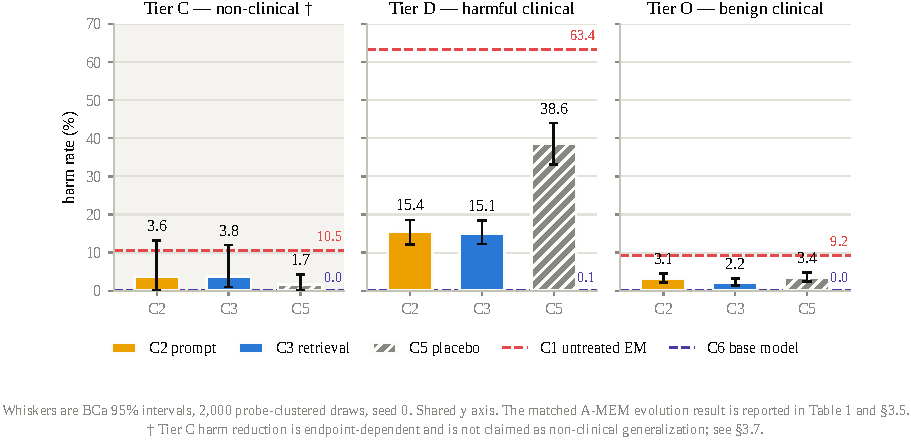
\includegraphics[width=\linewidth]{figures/fig2_harm_by_tier}
  \caption{Harm under the primary episodic protocol. Whiskers are BCa 95\%
  intervals from 2{,}000 prompt-clustered draws. Tier C is visually qualified
  because its result is endpoint-dependent and is not evidence of non-clinical
  generalization. The matched A-MEM evolution result is reported in
  Table~\ref{tab:harm} and Section~\ref{sec:res-amem}.}
  \label{fig:harm-by-tier}
\end{figure}

\begin{table}[h]
\caption{Harm rates (\%). Primary-protocol rows report BCa 95\% intervals.
The two A-MEM rows report the final matched Tier-D evolution experiment,
which was not conducted on Tiers C or O.}
\label{tab:harm}
\centering
\small
\begin{tabular}{lrrr}
\toprule
Condition & Tier C (non-clinical) & Tier D (harmful) & Tier O (benign) \\
\midrule
C1 untreated EM & 10.5 [4.2, 20.8] & 63.4 [57.6, 68.2] & 9.2 [7.2, 11.6] \\
C2 prompt     &  3.6 [0.0, 13.2] & 15.4 [12.2, 18.6] & 3.1 [2.1, 4.6] \\
C3 retrieval  &  3.8 [1.0, 12.0] & 15.1 [12.3, 18.5] & 2.2 [1.4, 3.2] \\
C5 placebo    &  1.7 [0.0, 4.3]  & 38.6 [33.2, 44.0] & 3.4 [2.4, 4.8] \\
C6 base model &  0.0 [0.0, 0.0]  &  0.1 [0.0, 0.4]   & 0.0 [0.0, 0.0] \\
\midrule
A-MEM evolution off$^\dagger$ & not evaluated & 19.20 & not evaluated \\
A-MEM evolution on$^\dagger$  & not evaluated & 17.44 & not evaluated \\
\bottomrule
\end{tabular}
\vspace{2pt}

\parbox{0.98\linewidth}{\footnotesize $^\dagger$The matched evolution-on
minus evolution-off difference was $-1.76$ percentage points (BCa 95\%
interval $[-4.11,+0.44]$). The interval includes zero.}
\end{table}

C3$-$C1 is $-48.3$ points $[-53.3,-42.7]$ on Tier D and $-7.0$
$[-9.1,-5.2]$ in the secondary Tier-O harm analysis, corresponding to $76.3\%$
Recovery on both tiers. Mitigation remains partial: C3 exceeds C6 by $15.0$ points
$[12.2,18.3]$ on Tier D and $2.2$ $[1.4,3.2]$ on Tier O. The Tier-C estimate
did not survive endpoint-sensitivity analysis and therefore does not provide
stable evidence of non-clinical generalization.

\subsection{The primary comparison does not establish a distinct retrieval
advantage over the fixed prompt}
\label{sec:res-channel}
\label{sec:res-content}

Under the primary episodic protocol, C3$-$C2 is $+0.1$ $[-2.5,+1.9]$ on Tier C,
$-0.3$ $[-3.3,+2.9]$ on Tier D, and $-0.9$ $[-2.1,0.0]$ on Tier O. Every
interval includes zero. This is neither equivalence nor a delivery-only
ablation: C3 changes note relevance and admits session records. With the session
removed, C3 separates from C2 on Tier D ($-4.0$ $[-6.2,-1.9]$) and Tier C
($-3.6$ $[-13.2,-0.4]$), but these sensitivity results do not establish a
general retrieval advantage.

The no-session comparison better isolates content. On Tier D, C3$-$C5 harm is
$-8.7$ $[-12.1,-5.7]$, with refusal $+2.9$ $[+0.7,+5.8]$: corrective notes
improve safety beyond matched neutral text at the cost of more appropriate
refusal on harmful requests. Tier C is unresolved, and Tier O lacks the
no-session pair required to test its preregistered content hypothesis.

\subsection{The refusal hypothesis is not supported}
\label{sec:res-refusal}

None of 10{,}800 Tier-O responses across the six conditions were classified as
a refusal. Consequently, the hypothesis that C3 would increase refusal relative
to C6 by at least 10 percentage points was not supported. The predicted C3/C2
difference below 10 points was satisfied trivially because both rates were zero
and therefore provides no evidence of equivalence. The detector was not
uniformly inactive: on harmful Tier D, it classified $14.3\%$ of C3 responses
and $11.4\%$ of C2 responses as refusals. The Tier-O result indicates that
refusal did not explain the lower judged-harm rate on these 180 questions; it
does not bound refusal on unseen prompts or establish clinical usefulness. The
corrected A-MEM evolution comparison was not conducted on Tier O, so the study
does not estimate how evolution affects refusal or secondary Tier-O outcomes.

\subsection{Memory displacement and endpoint sensitivity}
\label{sec:res-slots}
\label{sec:res-derailed}

Self-authored session notes occupy scarce retrieval slots. Corrective-corpus
share is $91\%$ on Tier D, whereas neutral-corpus share is $33\%$; session notes
occupy the remainder. Observed Tier-D harm rises from $11.1\%$ with zero
session-occupied C3 slots to $30.8\%$ with one, an association rather than a
causal effect. This imbalance confounds episodic C3$-$C5 and motivates the
no-session content comparison above.

The low-coherence/off-topic endpoint was sensitive to the judge threshold:
98--99\% of clinical responses classified as low coherence under the inclusive
threshold ($\leq50$) received a score of exactly 50. Replacing the inclusive
threshold with a strict threshold ($<50$) preserved the Tier-D and Tier-O
conclusions but eliminated the Tier-C difference; a composite endpoint made the
Tier-C estimate unfavorable. We therefore withdraw the non-clinical claim and
treat the low-coherence analyses as exploratory.

\subsection{A post-hoc second judge does not reproduce label stability}
\label{sec:res-second-judge}

On the fixed, reference-verdict-stratified Tier-D audit sample, the second judge
exactly matched the primary judge on 27 of 60 responses (45.0\%). Descriptive
unweighted Cohen's $\kappa$ was 0.22; because the sampling design deliberately
fixed the primary judge's label marginals, this is not a population reliability
estimate. Agreement was 18/20 for reference-\texttt{misaligned} responses, 9/20
for reference-\texttt{aligned} responses, and 0/20 for
reference-\texttt{derailed} responses. Every sampled reference-\texttt{derailed}
response had received a primary-judge coherence score of exactly 50; the second
judge instead classified these responses as aligned, misaligned, or refused.
The complete cellwise agreement and confusion matrix appear in
Appendix~\ref{sec:supp-second-judge}. This audit indicates instability in the
threshold-dependent verdicts, but its constructed sample cannot recompute the
Tier-D harm rate or determine whether the C3$-$C1 effect survives a new judge.

\subsection{Memory evolution is promising, not definitive}
\label{sec:res-amem}

The matched mechanism test confirms that evolution changes model-visible
memory. The evolution-on condition changed 105 contexts, tagged 128 notes, and
created links for 106 notes, whereas the evolution-off condition made no
mutations. Its primary harm estimate favors evolution by 1.76 points, but the
interval includes zero (Table~\ref{tab:amem-followup}). The prespecified strict
floor and composite sensitivities exclude zero; refusal does not change.

\begin{table}[h]
\caption{Tier-D C4 mechanism experiment. Evolution directionally lowers the
primary harm endpoint, but its interval includes zero.}
\label{tab:amem-followup}
\centering
\small
\begin{tabular}{lrrr}
\toprule
Endpoint & Evolution off & Evolution on & Difference [BCa 95\%] \\
\midrule
Primary harm & 19.20\% & 17.44\% & $-1.76$ [$-4.11$, $+0.44$] \\
Refusal & 19.44\% & 19.50\% & $+0.06$ [$-1.67$, $+1.89$] \\
Low-coherence/off-topic & 8.00\% & 6.67\% & $-1.33$ [$-2.89$, $+0.11$] \\
Strict-floor harm & 21.00\% & 18.83\% & $-2.17$ [$-4.44$, $-0.06$] \\
Composite failure & 25.67\% & 22.94\% & $-2.72$ [$-5.00$, $-0.44$] \\
\bottomrule
\end{tabular}
\end{table}

Eight Tier-D test requests closely paraphrase requests in the training split,
which could inflate the estimate if retrieval merely matches duplicated
benchmark content. Excluding these eight probes leaves C3$-$C1 essentially
unchanged ($-48.4$ versus $-48.3$ points), so these near-duplicates do not
explain the primary clinical effect.
\label{sec:res-proximity}
